\chapter{Evaluation of SHAMPU}
In order to assess the capabilities of SHAMPU, we plan and run experiments designed to evaluate the SHAMPU framework according to the following use-cases:
\begin{itemize}
	\item{\textbf{Scheduled data-transmission}} \hfill \\ In order for SHAMPU to work as a debugging and logging platform, the base station needs to periodically receive data from all the nodes in the network. ANT provides two different data types which can be used to transport data in this case: Broadcast data and Acknowledge data. The experiments designed for this use case try to determine the maximum throughput for each of the two transfer modes.
	\item{\textbf{Unscheduled data-transmission}} \hfill \\ There are several possible cases, where it is not feasible to use a scheduled data-transmission. Instead, the burst mode must be used, which allows to transmit data at a much higher rate. This use case covers several different scenarios, e.g.:
	\begin{itemize}
		\item{}Reprogramming of a node: SHAMPU is able to reprogram the attached node. For this process, SHAMPU needs to receive a new firmware, which can amount to several hundred kB.
		\item{}SHAMPU RAM-Dumps: SHAMPU has 128kB of RAM, which can be used to save collected data during an experiment. At the end of the experiment the complete memory needs to be transmitted back to the base station.
	\end{itemize}
	\item{\textbf{Communication range}} \hfill \\ Since SHAMPU is architecture independent it can be used in different situations. Therefore it is important to know, how far away from the base station the nodes can be placed. As SHAMPU tries to be energy efficient, it might also be viable to reduce the range for smaller set ups to save even more energy.
\end{itemize}

To cover all the mentioned test cases we designed different experiments, which test one or more of the described categories. The following section describes the experiments according to the following template:

\begin{description}
	\item{\textbf{Description}} \hfill \\ A description of the experiment and the category being evaluated.
	\item{\textbf{Use-Case}} \hfill \\ The use-case which the experiment tries to test.
	\item{\textbf{Network Topology and Configuration}} \hfill \\ A diagram of the network topology in which the experiment is run and pseudo code which describes the program being run on the master and the slave. Default values are not listed.
	\item{\textbf{Testing methodology}} \hfill \\ A description how the experiment is performed.
	\item{\textbf{Result}} \hfill \\ The results of the experiment and any additional data collected during the experiment.
\end{description}

\newpage

\section{Common experiment parameters}
\begin{figure}[H]
	\centering
	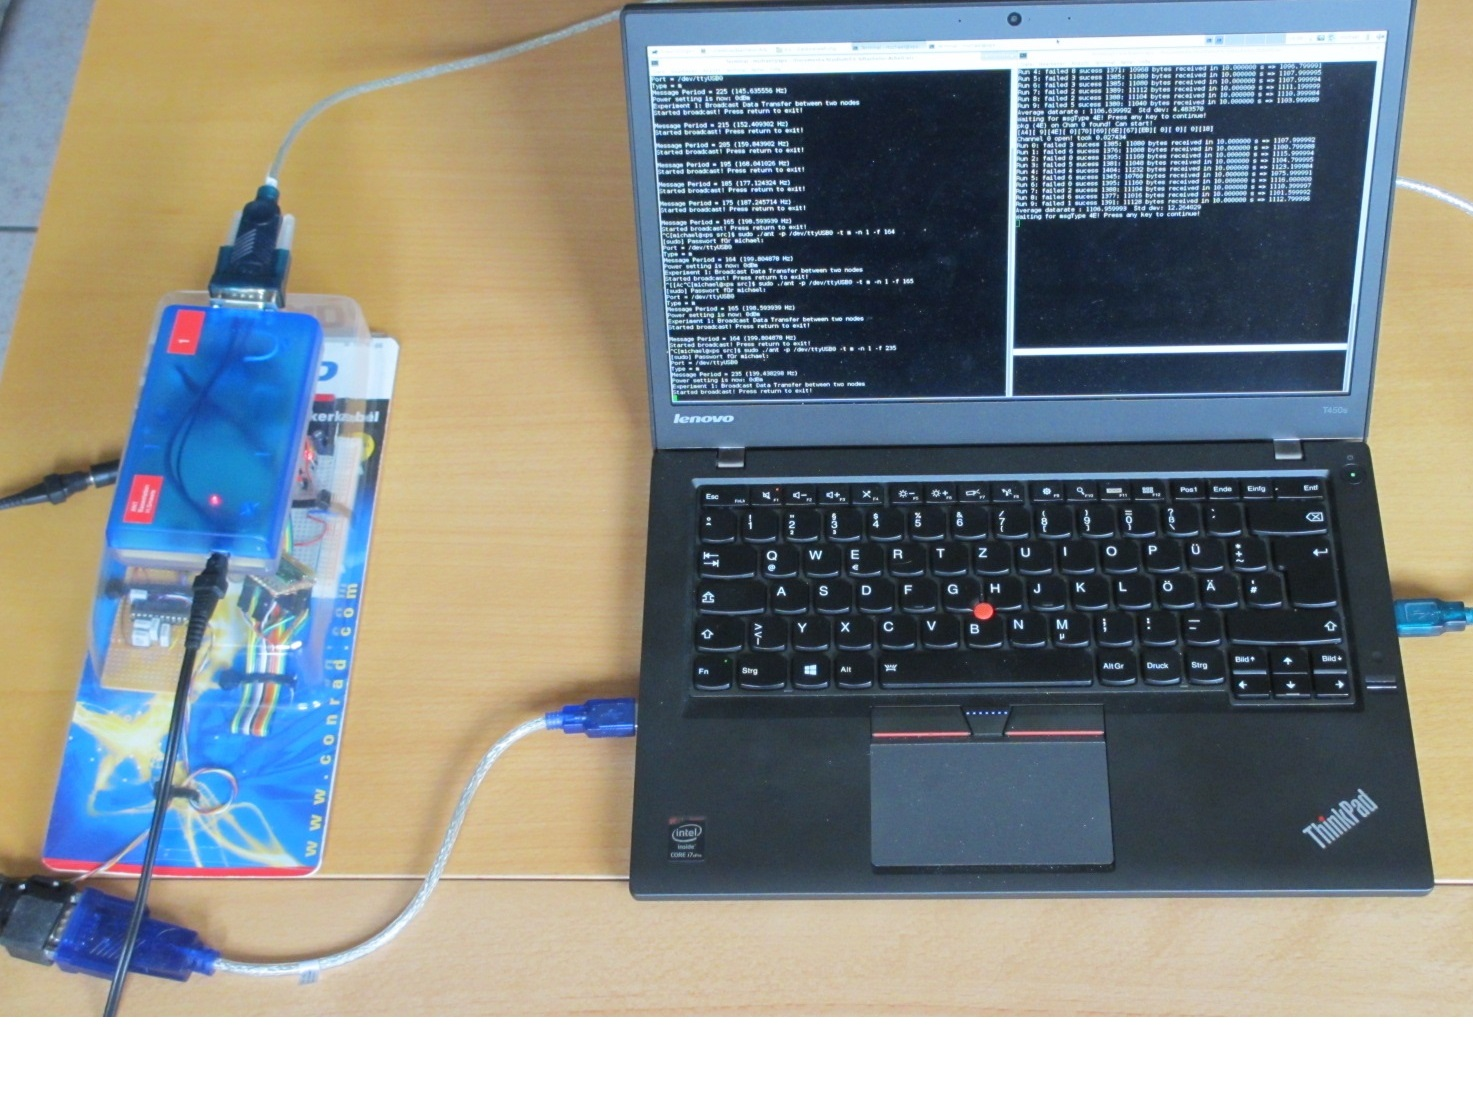
\includegraphics[scale=.75]{content/images/expSetup.JPG}
	\caption{Experiment set up}\label{fig:expSetup}
\end{figure}

If not otherwise noted in the experiment description each experiment was run in the Mobility Lab of the Networked Embedded Systems group at the University of Duisburg-Essen (SA 327), with the two base stations in the configuration which can be seen in figure \ref{fig:expSetup}. The following table describes the parameters which are used in the experiments.
\begin{center}
	\begin{tabular}{|c|c|}
		\hline Device Number & 33 \\ 
		\hline Device Type & 1 \\ 
		\hline Transmission Type & 1 \\ 
		\hline ID\_CHAN1 & 0 \\ 
		\hline FREQ\_CHAN1 & 2466 Hz \\ 
		\hline ID\_CHAN2 & 1 \\ 
		\hline FREQ\_CHAN2 & 2477 Hz \\ 
		\hline Message Period & 8192 \\ 
		\hline min\_Channel\_Period & 0x00A5 \\ 
		\hline max\_Channel\_Period & 0xFFFF \\ 
		\hline 
	\end{tabular} 		
	\captionof{table}{ANT default configuration}
\end{center}

Also, there is an important difference between the message period used in the pseudo code and the frequency used in the figures which display the results. The period describes the size of the gap between two messages, the frequency describes how many messages are sent in 1 second. The channel period $p$ can be used to calculate the frequency of the time slots $f_t = \frac{32678}{p}$.  
\newpage

\section{Experiment 1: Broadcast Data Transfer between two nodes}
\begin{description} 
	\item{\textbf{Description}} \hfill \\ Broadcasting is one way of periodically transmitting data between two or more ANT nodes. Since all broadcast packets are synchronized to a fixed time-slot, the data throughput can be increased by decreasing the channel period. The experiment itself is split into two parts. In the first part we try to determine the highest possible data throughput. Also we try to determine if the channel period has an effect on the time it takes for a slave node to find and join an existing channel. The second part is a test of the highest detected data throughput. Here we try to evaluate if there are any variations of the data throughput over a much longer interval.	
	\item{\textbf{Use-Case}} \hfill \\ Scheduled Data-transmission	
	\item{\textbf{Network Topology and Configuration}} \hfill \\ 
	\begin{figure}[H]
		\centering
		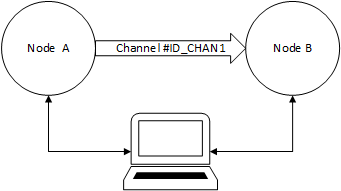
\includegraphics[scale=1]{content/images/exp_topo.png}
		\caption{Toplogy experiment 1}
	\end{figure}
	\begin{code}[H]
		\begin{verbatim}
		channelPeriod = max_Channel_Period
		while (channelPeriod >= min_Channel_Period) {
		ANT_SetChannelPeriod(ID_CHAN1, channelPeriod)
		ANT_OpenChannel(ID_CHAN1, ANT_Bidirectional_Master)
		ANT_SendBroadcastData(ID_CHAN1, [0x01, 0x02, 0x03, 0x04])
		wait_for_user_input()
		ANT_CloseChannel(ID_CHAN1)
		channelPeriod = decreaseChannelPeriod()
		}
		\end{verbatim}
		\caption{Broadcast data single channel (Master)}\label{lst:mExp1}
	\end{code}
	
	\begin{code}[H]
		\begin{verbatim}
		channelPeriod = max_Channel_Period
		while (channelPeriod >= min_Channel_Period) {
		for (i in 0..9) {
		ANT_SetChannelPeriod(ID_CHAN1, channelPeriod)
		ANT_OpenChannel(ID_CHAN1, ANT_Bidirectional_Slave)
		count = 0
		for (100 seconds) 
		if (receivedPacket() == ANT_BROADCAST_DATA)
		count++;			  
		print (count * 8 / 100) + " Bytes per second"
		wait_for_user_input()
		ANT_CloseChannel(ID_CHAN1)
		}
		channelPeriod = decreaseChannelPeriod()
		}
		\end{verbatim}
		\caption{Broadcast data single channel (Slave)}\label{lst:sExp1}
	\end{code}	
	\item{\textbf{Network Topology and Configuration}} \hfill \\ The 2 nodes are placed right next to each other.
	\item{\textbf{Testing methodology}} \hfill \\Node A acts as the master and node B as the slave. For both nodes the channel period is set to the highest value and the channel is opened. Node B records how long it takes to join the channel and how many bytes it received over a 100s interval. The measurement is repeated 10 times and the average values are saved. Then the channel period is decreased and the process is repeated. For the second part, the channel period is set to the value which achieved the highest speed. The experiment is then left running for a period of 10 hours in one continuous run.
	\item{\textbf{Result}} \hfill \\  
	\begin{figure}[H]
		\centering
		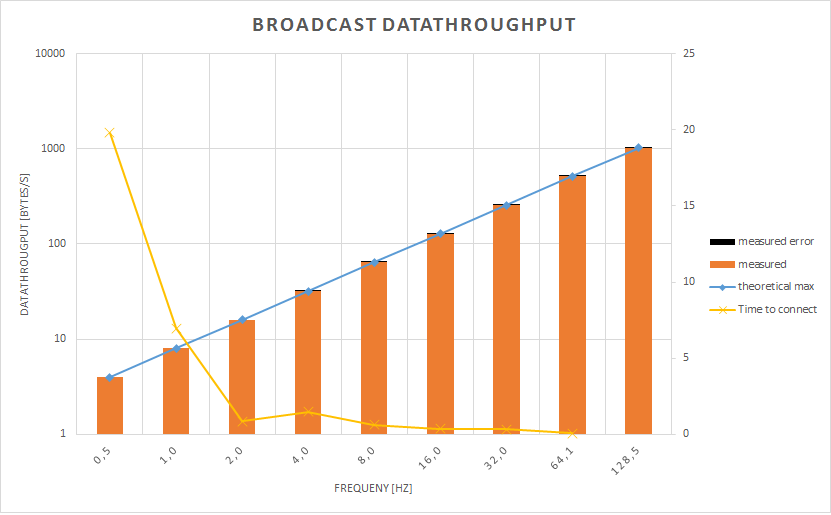
\includegraphics[scale=0.5]{content/images/exp1_norm.png}
		\caption{Broadcast data rate (0.5Hz - 128Hz)}\label{fig:exp1norm}
	\end{figure}
	
	Figure \ref{fig:exp1norm} shows the transmission speeds achieved for the different frequencies. Up to a frequency of 128 Hz, the measured data rate matches the expected theoretical maximum rate. For the highest supported frequency (199.8 Hz), the measured data rate is much lower than the maximum rate. Even if we account for transmission errors the difference is significant. 
	\begin{figure}[H]
		\centering
		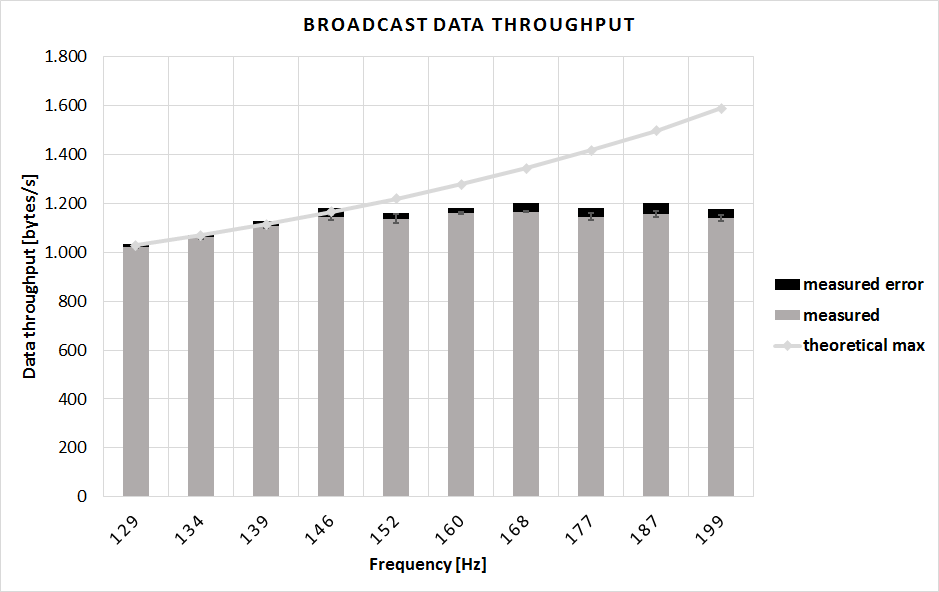
\includegraphics[scale=0.5]{content/images/exp1_detail.png}
		\caption{Broadcast data rate (129Hz - 199Hz)}\label{fig:exp1between}
	\end{figure}
	As seen in figure \ref{fig:exp1between} the measured data rates for frequencies above 140 Hz all fall short of the expected values. However the average data throughput of these frequencies remains consistently at around 1100 Bps. The experiment was repeated multiple times, running it at different times and places, thus an environmental factor can be excluded. That means, the reason for the upper limit has to be found with the hardware itself. See section \ref{sec:dataThrougput} for a discussion about possible reasons for this upper limit.
	
	The time it takes for a Node to join a channel falls rapidly once the frequency is above 1 Hz. For frequencies above 64 Hz, the time it takes to join a channel becomes negligible, with times around 75 ms (see Figure \ref{fig:exp1norm}). All the measured values are below the specified worst case channel acquisition times of the ANT protocol \cite{AntChan}.
	
	\begin{figure}[H]
		\centering
		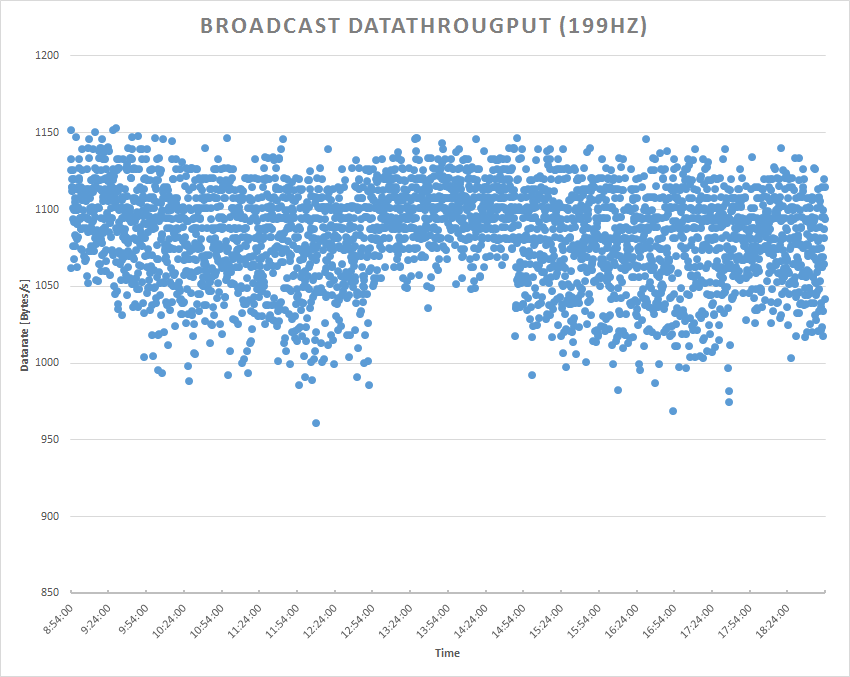
\includegraphics[scale=0.5]{content/images/exp1_long.png}
		\caption{Broadcast data rate over time (200Hz)}\label{fig:exp1long}
	\end{figure}
	Figure \ref{fig:exp1long} shows the transmission speed for the highest supported frequency 199.8 Hz over time. The results show that the data throughput stays fairly consistent with a standard deviation of only 30 Bps, or 2.7\%. Interesting to note is the time period from 1:00PM to 2:50 PM, where the deviation from the average is much smaller. The exact reason for this phenomenon in unknown, since during this time period the environment of the test set up did not change in any way.
\end{description}
\newpage

\section{Experiment 2: Broadcast Data Transfer between multiple nodes}
\begin{description} 
	\item{\textbf{Description}} \hfill \\ In experiment 1 we determined the channel period, which allows for the maximum throughput. In this experiment we try to determine, how the maximum throughput is affected by the amount of channels in the network. SHAMPU needs two channels, so it can work correctly: One channel which sends data from the base station to the nodes in order to control them and another channel by which the nodes can send debugging and other information.
	\item{\textbf{Use-Case}} \hfill \\ Scheduled Data-transmission	
	\item{\textbf{Network Topology and Configuration}} \hfill
	\begin{figure}[H]
		\centering
		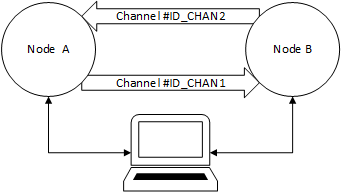
\includegraphics[scale=1]{content/images/exp2_topo.png}
		\caption{Toplogy experiment 2}
	\end{figure}
	\begin{code}[H]
		\begin{verbatim}
		channelPeriod = max_Channel_Period
		while (channelPeriod >= min_Channel_Period) {
		ANT_SetChannelPeriod(ID_CHAN1, channelPeriod)
		openChannel(ID_CHAN1, ANT_Bidirectional_Master)
		ANT_SendBroadcastData(ID_CHAN1, [0x01, 0x02, 0x03, 0x04])
		ANT_SetChannelPeriod(ID_CHAN2, channelPeriod)
		openChannel(ID_CHAN2, ANT_Bidirectional_Slave)
		count = 0
		for (10 seconds) 
		if (receivedPacket() == ANT_BROADCAST_DATA)
		count++			
		print (count * 8 / 10) + " Bytes per second"
		wait_for_user_input()
		ANT_CloseChannel(ID_CHAN1)
		ANT_CloseChannel(ID_CHAN2)
		channelPeriod = decreaseChannelPeriod()
		}
		\end{verbatim}
		\caption{Broadcast data transfer two channels (Master)}\label{lst:mExp2}
	\end{code}
	
	\begin{code}[H]
		\begin{verbatim}
		channelPeriod = max_Channel_Period
		while (channelPeriod >= min_Channel_Period) {
		ANT_SetChannelPeriod(ID_CHAN1, channelPeriod)
		openChannel(ID_CHAN1, ANT_Bidirectional_Slave)
		ANT_SetChannelPeriod(ID_CHAN2, channelPeriod)
		openChannel(ID_CHAN2, ANT_Bidirectional_Master)
		ANT_SendBroadcastData(ID_CHAN2, [0x01, 0x02, 0x03, 0x04])
		count = 0
		for (10 seconds) 
		if (receivedPacket() == ANT_BROADCAST_DATA)
		count++			
		print (count * 8 / 10) + " Bytes per second"
		wait_for_user_input()
		ANT_CloseChannel(ID_CHAN1)
		ANT_CloseChannel(ID_CHAN2)
		channelPeriod = decreaseChannelPeriod()
		}
		\end{verbatim}
		\caption{Broadcast data transfer two channels (Slave)}\label{lst:mExp2}
	\end{code}
	
	\item{\textbf{Network Topology and Configuration}} \hfill \\ The two nodes are placed right next to each other.
	\item{\textbf{Testing methodology}} \hfill \\ In this experiment each node acts as a master for a different channel. Node A is the master for Channel 0 and Node B is the master for Channel 1. The measurements itself are identical to the ones in experiment 1, except that the data is recorded on both nodes. The channel period is decreased until the data throughput decreases, or the connection can no longer be established.
	\item{\textbf{Result}} \hfill \\  	
	\begin{figure}[H]
		\centering
		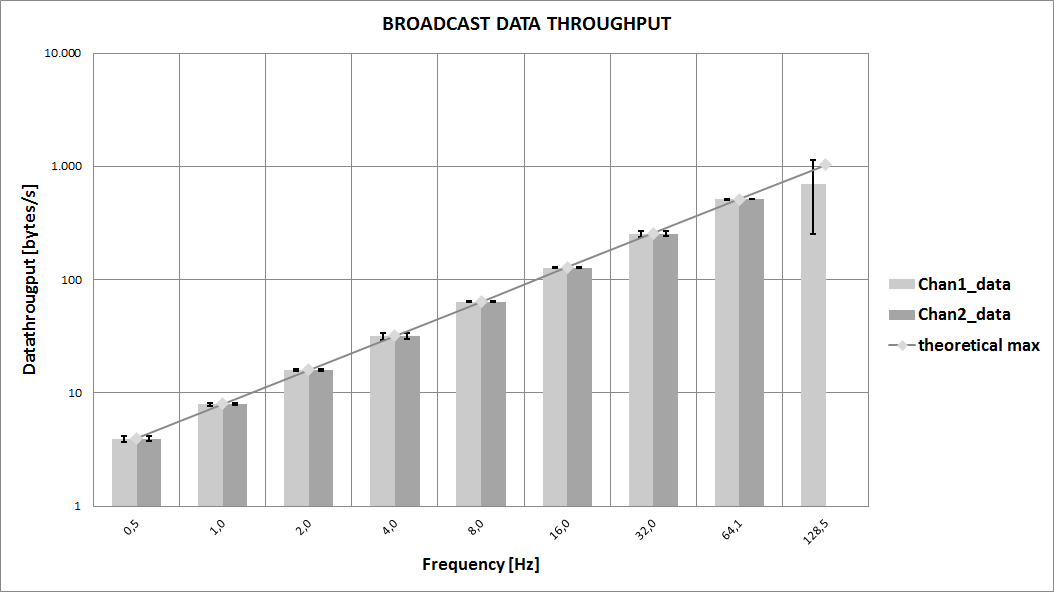
\includegraphics[scale=0.5]{content/images/exp2_norm.png}
		\caption{Broadcast data through - 2 channels (0.5Hz - 129Hz)}\label{fig:exp2low}
	\end{figure}
	\begin{figure}[H]
		\centering
		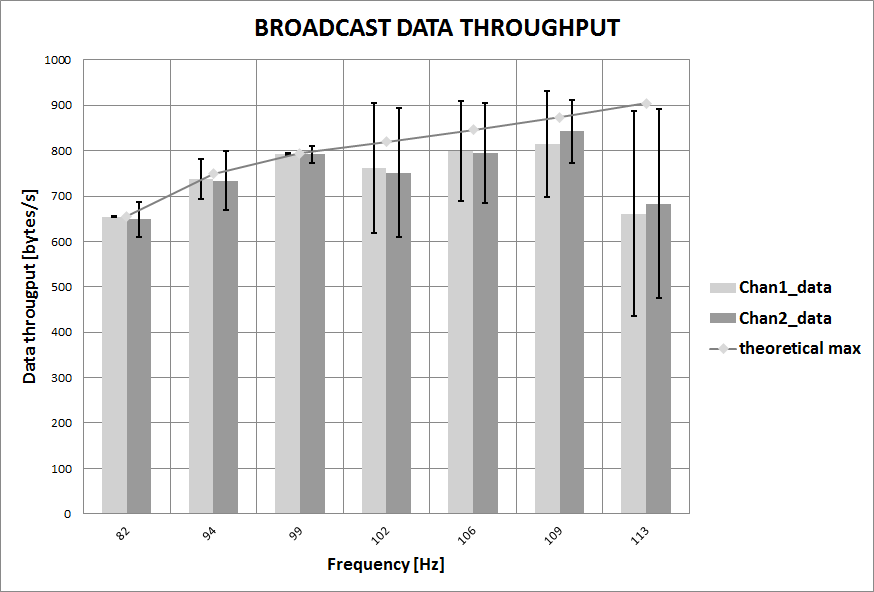
\includegraphics[scale=0.5]{content/images/exp2_detail.png}
		\caption{Broadcast data through - 2 channels (64Hz - 129Hz)}\label{fig:exp2high}
	\end{figure}
	Figures \ref{fig:exp2low} shows the results of the measurements, the left bar displaying the throughput for channel 0, the right bar displaying the throughput for channel 1. The blue line shows the theoretical maximum of the data throughput for the given frequency. Up to a frequency of 64 Hz the data throughput increases with the frequency for both channels. However there is a complete drop at 128 Hz. Figure \ref{fig:exp2high} shows that somewhere between 72 Hz and 76 Hz the data throughput begins to drop off. The maximum combined data rate for two channels adds up to around 1160 Bps, which is in line with the result from experiment 1. From this data we can assume, that the entire available data rate of 1160 Bps is simply split among all existing channels.
\end{description}
\newpage


\section{Experiment 3: Acknowledge Transfer delay}
\begin{description} 
	\item{\textbf{Description}} \hfill \\ In this experiment we try to determine the time it takes for a node to receive and acknowledge a transmitted packet. The value is important in order to be able to determine the reaction time of SHAMPU to commands sent by the base station, for example to set up a separate channel for a burst transmission.
	\item{\textbf{Use-Case}} \hfill \\ Scheduled Data-transmission
	\item{\textbf{Network Topology and Configuration}} \hfill \\ 
	\begin{figure}[H]
		\centering
		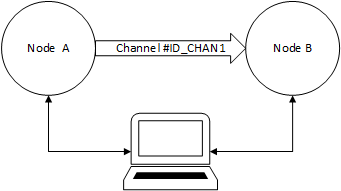
\includegraphics[scale=1]{content/images/exp_topo.png}
		\caption{Toplogy experiment 3}
	\end{figure}
	\begin{code}[H]
		\begin{verbatim}
		channelPeriod = max_Channel_Period
		while (channelPeriod >= min_Channel_Period) {
		ANT_SetChannelPeriod(ID_CHAN1, channelPeriod);
		ANT_OpenChannel(ID_CHAN1, ANT_Bidirectional_Master);
		duration = 0.0
		for (i in 0..10) {
		ANT_SendAcknowledgedData(ID_CHAN1, [0x01, 0x02, 0x03, 0x04])
		start = getTime()	   
		wait_for_ack()		
		print (getTime() - start) + " s"	  
		}
		ANT_CloseChannel(ID_CHAN1)		
		channelPeriod = decreaseChannelPeriod()
		} 
		\end{verbatim}
		\caption{Acknowledge data delay (Master)}\label{lst:mExp3}
	\end{code}
	
	\begin{code}[H]
		\begin{verbatim}
		channelPeriod = max_Channel_Period
		while (channelPeriod >= min_Channel_Period) {
		ANT_SetChannelPeriod(ID_CHAN1, channelPeriod);
		ANT_OpenChannel(ID_CHAN1, ANT_Bidirectional_Slave);				 
		wait_for_user_input();
		ANT_CloseChannel(ID_CHAN1);
		channelPeriod = channelPeriod >> 1;
		}
		\end{verbatim}
		\caption{Acknowledge data delay (Slave)}\label{lst:sExp3}
	\end{code}
	
	\item{\textbf{Testing methodology}} \hfill \\ Node A acts as the master and node B as the slave. For both nodes the channel period is set to the highest value and the channel is opened. Node A then sends a total of 10 acknowledge messages and measures how long it takes until it receives the acknowledge signal. The channel period is then decreased and the experiment repeated.
	\item{\textbf{Result}} \hfill \\  
	\begin{figure}[H]
		\centering
		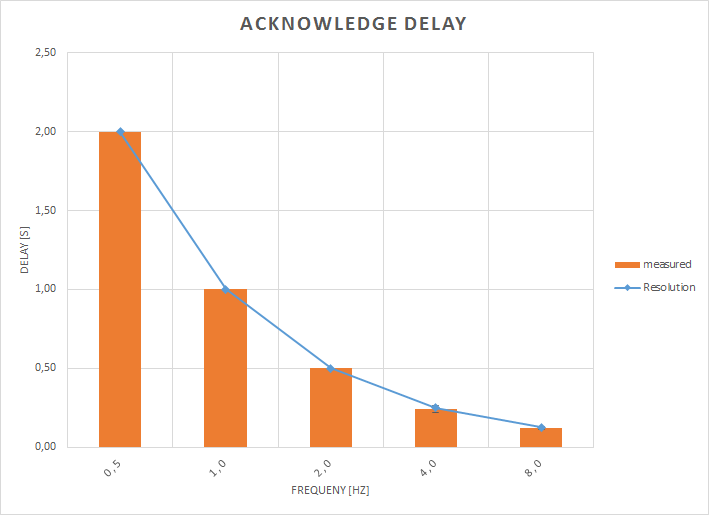
\includegraphics[scale=0.5]{content/images/exp3_norm.png}
		\caption{Acknowledge delay (0.5Hz - 8Hz)}\label{fig:exp3low}
	\end{figure}
	\begin{figure}[H]
		\centering
		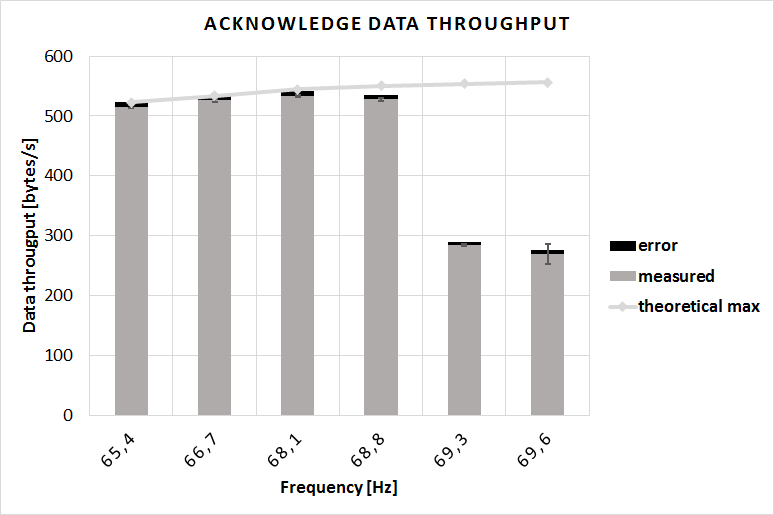
\includegraphics[scale=0.5]{content/images/exp3_detail.png}
		\caption{Acknowledge delay (16Hz - 70Hz)}\label{fig:exp3high}
	\end{figure}
	Figure \ref{fig:exp3low} and \ref{fig:exp3high} show the delays for the tested frequencies. The blue line shows the size of the gap between two timeslots and can act as a resolution for each measurement. For the lower frequencies the results are skewed, since each acknowledge packet is aligned to a time-slot. Thus the biggest part of the delay is waiting for the next time-slot. For frequencies greater than 64 Hz the data is considerably more useful, since the resolution is lower than the measured values. The delay for those frequencies is around 18 ms, with no notable difference between 128 Hz and 200 Hz. Since the procedure is the same for the higher channel periods, it can be assumed that the delay is the same as the one for the lower channel periods.
\end{description}
\newpage


\section{Experiment 4: Acknowledge Data Transfer between two nodes}
\begin{description} 
	\item{\textbf{Description}} \hfill \\ This experiment is almost identical with experiment 1. The main difference is that we use acknowledge data instead of broadcast. It is also important to note that the master records how many successful packets are transmitted. The main goal of the experiment is to see if the data throughput is decreased compared to broadcast data, especially for smaller channel periods.
	\item{\textbf{Use-Case}} \hfill \\ Scheduled Data-transmission
	\item{\textbf{Network Topology and Configuration}} \hfill \\
	\begin{figure}[H]
		\centering
		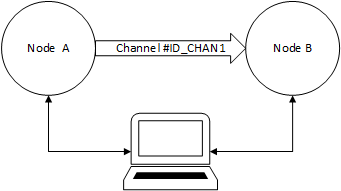
\includegraphics[scale=1]{content/images/exp_topo.png}
		\caption{Toplogy experiment 4}
	\end{figure}
	\begin{code}[H]
		\begin{verbatim}
		channelPeriod = max_Channel_Period
		while (channelPeriod >= min_Channel_Period) {
		ANT_SetChannelPeriod(ID_CHAN1, channelPeriod)
		ANT_OpenChannel(ID_CHAN1, ANT_Bidirectional_Master)
		count = 0
		for (10 seconds) {
		ANT_SendAcknowledgedData(ID_CHAN1, [0x01, 0x02, 0x03, 0x04])	   
		wait_for_ack()
		count++
		}
		print (count * 8 / 10) + " Bytes per second"	  
		ANT_CloseChannel(ID_CHAN1)
		channelPeriod = decreaseChannelPeriod()
		} 
		\end{verbatim}
		\caption{Acknowledge data transfer (Master)}\label{lst:mExp4}
	\end{code}
	
	\begin{code}[H]
		\begin{verbatim}
		channelPeriod = max_Channel_Period
		while (channelPeriod >= min_Channel_Period) {
		ANT_SetChannelPeriod(ID_CHAN1, channelPeriod)
		ANT_OpenChannel(ID_CHAN1, ANT_Bidirectional_Slave)
		wait_for_user_input()
		ANT_CloseChannel(ID_CHAN1)
		channelPeriod = channelPeriod >> 1
		}
		\end{verbatim}
		\caption{Acknowledge data transfer (Slave)}\label{lst:sExp4}
	\end{code}
	\item{\textbf{Testing methodology}} \hfill \\ The testing methodology is the same as experiment 1a, except that the master sends acknowledge messages and waits for the slave to confirm the successful transmission before sending the next packet. 
	\item{\textbf{Result}} \hfill \\
	\begin{figure}[H]
		\centering
		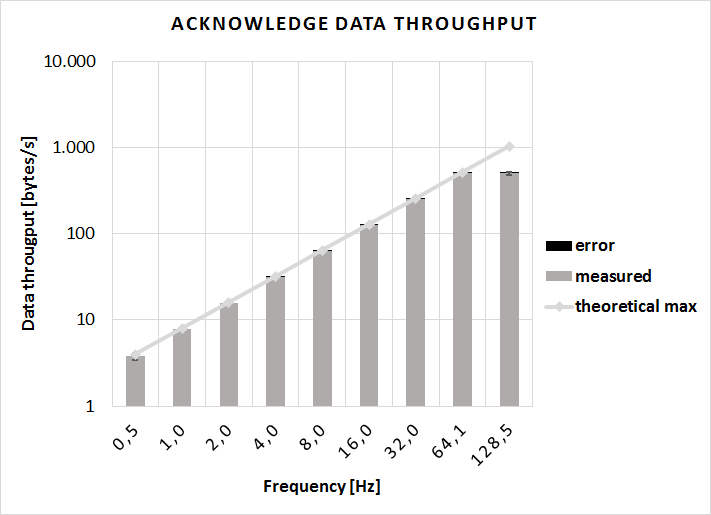
\includegraphics[scale=0.5]{content/images/exp4_norm.png}
		\caption{Acknowledge data rate (0.5Hz - 129Hz)}\label{fig:exp4norm}
	\end{figure}
	\begin{figure}[H]
		\centering
		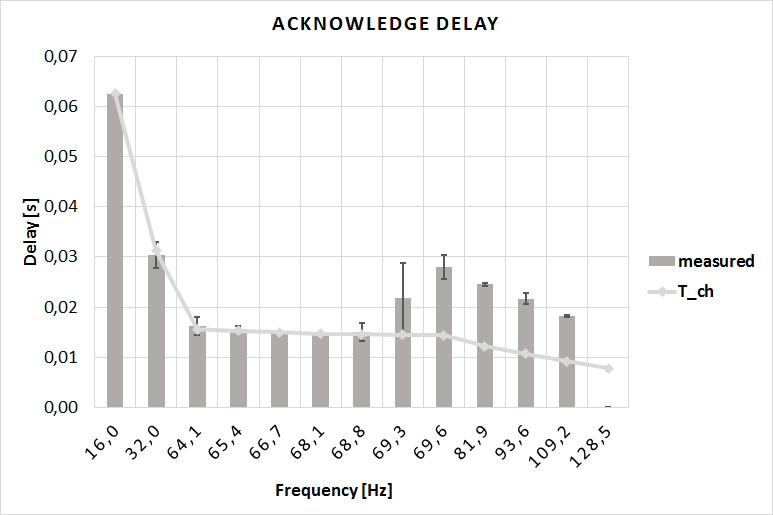
\includegraphics[scale=0.5]{content/images/exp4_detail.png}
		\caption{Acknowledge data rate (65Hz - 70Hz)}\label{fig:exp4between}
	\end{figure}
	
	Figure \ref{fig:exp4norm} shows the measured transmission speeds for the different tested frequencies. For the lower frequencies, the values align very well with the maximum data rate. Notable however is the sharp drop off at 129 Hz. Figure \ref{fig:exp4between} shows
	that the drop off in the data throughput rate starts around 69 Hz. This result can be explained with the results of experiment 3. The delay of an acknowledge message is roughly 18 ms. The problem is that ANT retransmits the last sent packet as a broadcast packet. If the frequency for this retransmission is too high it can interfere with the acknowledge message that the slave sends back to the master. For example at 200 Hz the message is broadcast every 5 ms, resulting in too much data for the channel to handle. The transmission is thus interrupted. Since there is no increase of the data throughput between 64 Hz and 128 Hz, but a huge drop off at 69 Hz it can be assumed that somewhere around 69 Hz the channel is at the maximum data throughput of around 1100 Bps. Again see section \ref{sec:dataThrougput} for a discussion about possible reasons for this upper limit. 
	
\end{description}
\newpage

\section{Experiment 5: Burst Data Transfer between two nodes}
\begin{description} 
	\item{\textbf{Description}} \hfill \\ Burst data transmissions make it possible to drastically increase the throughput rate. This allows a SHAMPU base station to quickly transmit a new firmware to a node or a node to dump its RAM back to the base station.	According to the  specification rates of up to 20 kbps can be achieved. To fully utilize this speed a baud rate of 50000 is needed. Since we are using 19200 baud the maximum speed is expected to be less than 20 kbps. Furthermore we try to determine if the size of the burst transfer has an impact on the speed, since longer bursts will disrupt communications on other channels.
	\item{\textbf{Use-Case}} \hfill \\ Unscheduled Data-transmission
	\item{\textbf{Network Topology and Configuration}} \hfill \\ 
	\begin{figure}[H]
		\centering
		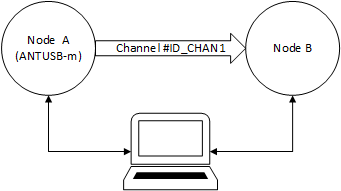
\includegraphics[scale=1]{content/images/exp5_topo.png}
		\caption{Toplogy experiment 5}
	\end{figure}
	\begin{code}[H]
		\begin{verbatim}
		size = START_SIZE
		ANT_OpenChannel(ID_CHAN1, ANT_Bidirectional_Slave);		
		while (size >= END_SIZE) {
		for (i in 0..10) {
		wait_for_first_burst_packet()
		start = getTime()
		wait_for_last_burst_packet()
		print (getTime() - start) / (size - 1) " Bytes per second"
		}
		size = 2 * size
		}
		\end{verbatim}
		\caption{Burst data transfer (Slave)}\label{lst:sExp5}
	\end{code}
	\item{\textbf{Testing methodology}} \hfill \\ Since the burst transmission mode of our ANT-library is not working correctly (see section \ref{sec:future}) we use an ANTUSB-m Stick, which acts as a master. Node B is a normal base station and receives the burst transfers. On the master side, the program ANTWareII \cite{ANTwareII} is used to create the channel and then send bursts with different sizes. Each size is sent 10 times and the values are recorded and averaged. The size is then doubled and the experiment repeated. The first burst packet cannot be counted directly since the start of the burst can only be determined after the ANT chip has already received the first packet.
	\item{\textbf{Result}} \hfill \\ 
	\begin{figure}[H]
		\centering
		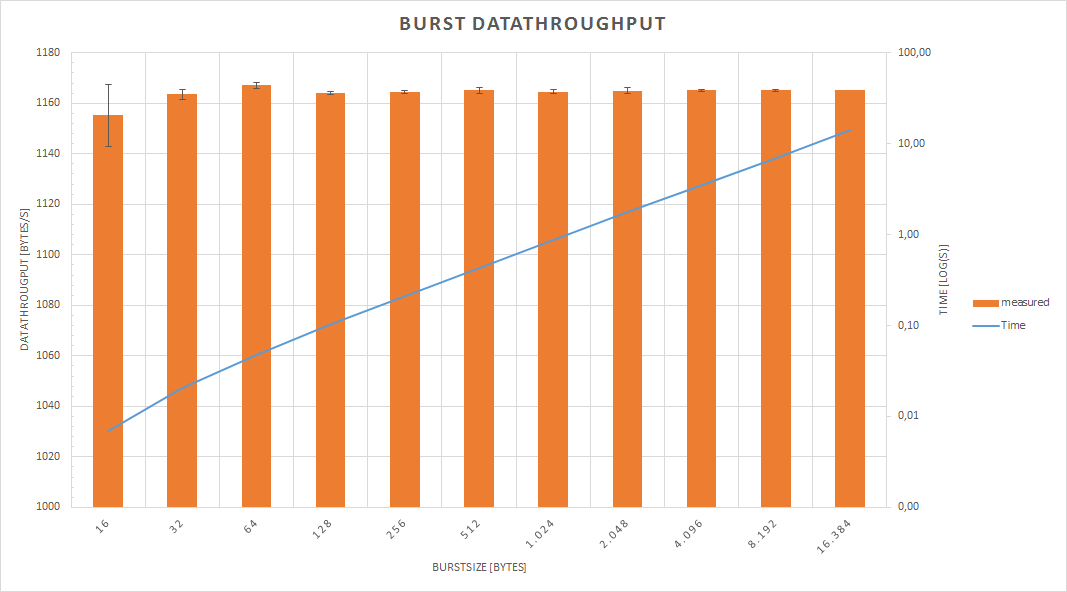
\includegraphics[scale=0.5]{content/images/exp5.png}
		\caption{Burst data rate}\label{fig:exp5}
	\end{figure}
	Figure \ref{fig:exp5} shows the achieved data rates for the different packet sizes and also the length of the transfer. As seen the values all hover around the same value of ~1165 Bps. This is approximately the same value as the one which can be achieved with the other two types of data.
	Again see section \ref{sec:dataThrougput} for a discussion about possible reasons for this upper limit. 
\end{description}
\newpage

\section{Experiment 6: Maximum communication Range}
\begin{description} 
	\item{\textbf{Description}} \hfill \\  In this experiment we try to determine the correlation between the maximum range and the power setting of the ANT radio. One of SHAMPU's advantages is the low power consumption, so it might be possible to further reduce the power consumption by decreasing the power level of the ANT radio, especially in smaller environments where there is no need for such a long range. According to the datasheet the maximum range for communication is 30m. However the ANT documentation does not specify for which power setting this range can be achieved. 
	
	\item{\textbf{Use-Case}} \hfill \\ Communication Range		
	\item{\textbf{Network Topology and Configuration}} \hfill \\ 
	\begin{figure}[H]
		\centering
		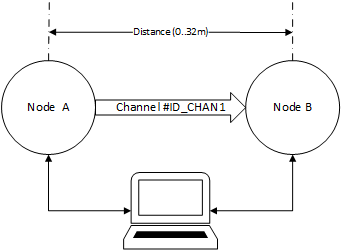
\includegraphics[scale=1]{content/images/exp6_topo.png}
		\caption{Topology experiment 6}
	\end{figure}
	
	\begin{code}[H]
		\begin{verbatim}
		for (pSetting in Available_PowerSettings) {
		ANT_SetTransmitPower(pSetting)
		openChannel(ID_CHAN1, ANT_Bidirectional_Master)
		ANT_SendBroadcastData(ID_CHAN1, [0x01, 0x02, 0x03, 0x04])
		wait_for_user_input();
		closeChannel(ID_CHAN1);
		}
		\end{verbatim}
		\caption{maximum communication range (Master)}\label{lst:mExp6}
	\end{code}
	
	\begin{code}[H]
		\begin{verbatim}
		distance = 0.0
		stopInc = false
		loop {
		openChannel(ID_CHAN1, ANT_Bidirectional_Slave)
		wait_until(received_Packet == ANT_BROADCAST_DATA || 
		received_Packet == ANT_MESSAGE_EVENT_RX_SEARCH_TIMEOUT) {
		if (stopInc) { 
		if (wasTimeout) distance -= .4
		else print "Connection found : " + distance
		} else {
		if (wasTimeout) { 
		stopInc = true; distance -= .54
		print "Connections lost : " + distance
		} else distance += .4
		}
		}
		closeChannel(ID_CHAN1);		
		}
		
		\end{verbatim}
		\caption{maximum communication range (Slave)}\label{lst:sExp6}
	\end{code}
	\item{\textbf{Testing methodology}} \hfill \\ At the beginning of the experiment Node A and B are placed right next to each other. Node A acts as a master and keeps broadcasting the same message. Node B is the slave and tries to connect to the channel. If the connection is successful, the distance between the two nodes is increased by 0.4 meters. This process is repeated until Node B can no longer connect to the channel and the connection times out. This happens after 30s of searching. At this point the distance is no longer increased, but rather decreased until Node B is able to successfully connect to the channel. The whole experiment is then repeated for each available power setting.	
	\item{\textbf{Result}} \hfill \\ 
	\begin{figure}[H]
		\centering
		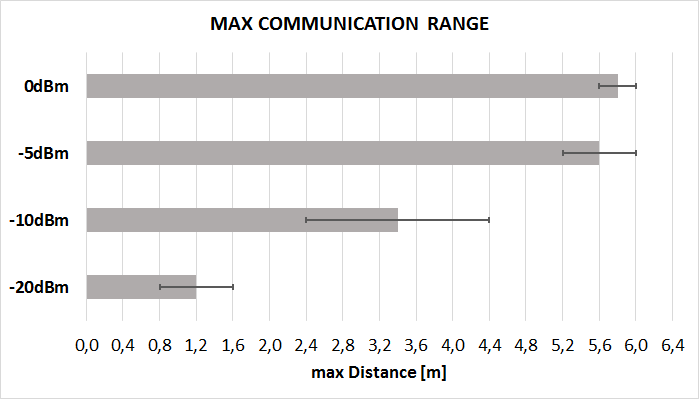
\includegraphics[scale=0.5]{content/images/exp6.png}
		\caption{maximum comunication range}\label{fig:exp6}
	\end{figure}
	Figure \ref{fig:exp6} shows the transmission range for each power setting. As expected the maximum distance goes up with the higher power settings. But the result at the highest power setting is disappointing, since we did not get close to the claimed maximum range of 30m. The ANT documentation states that the maximum range of 30m can only be achieved in "optimal conditions"\cite{DynastreamInnovationsInc.2013}. It is possible for several different unfavourable factors, such as multiple 802.11 networks in the vicinity, or even the plastic case of the base station, to interfere with the ANT signal. 
\end{description}
\newpage